\subsection{Literature-informed prey growth rates}\label{sec:literature-cases}
Following \citet[Sec.~4, Table~6]{haque11}, we use the prey growth rates attributed to
\citet{tanner75}. Table~\ref{tab:lit-rates} separates the reported observed rates from
Tanner's estimates for optimal conditions. For all three species pairs we use
\(k=100,\ \alpha=0.04,\ m=1.20,\ \beta=10,\ e=0.25,\ d=0.30\), with time in years.
The choices of \(k\) and \(d\) match values used in Haque's numerical setup. The other
common inputs define a controlled comparison for Eq.~\eqref{eq:ode}. Tanner's predator
growth rates describe population increase and do not enter the mortality parameter \(d\).

\begin{table}[htbp]
\centering\small
\caption{Prey growth-rate intervals and results at the lower observed endpoint. Rate intervals
and the largest eigenvalue real part are in \(\mathrm{yr}^{-1}\). Tanner's maximum estimates
represent optimal conditions.}\label{tab:lit-rates}
\begin{tabular}{@{}lccccc@{}}
\toprule
Prey / predator & Observed & Maximum & \((x^*,y^*)\) & \(\max\Re\lambda\) & Type \\
\midrule
Muskrat / mink & 0.806--1.068 & 1.101--1.366 & (65.009, 55.009) & \(-0.30939\) & Node \\
Moose / wolf & 0.100--0.127 & 0.171--0.202 & (11.200, 1.200) & \(-0.00429\) & Focus \\
Snowshoe hare / lynx & 0.545--0.810 & 0.769--1.033 & (34.207, 24.207) & \(-0.08160\) & Focus \\
\bottomrule
\end{tabular}
\end{table}

The common inputs give \(R=10\), \(C=12\), \(C_{\rm crit}=6.25r\), and
\(d-m\chi(4)=0.06\). At the largest listed rate \(C_{\rm crit}=8.5375\), so the
unique-root and cycle-exclusion conditions guarantee global convergence throughout all
six intervals. The phase portraits in Fig.~\ref{fig:lit-rates} show a node for
muskrat/mink and damped oscillations for the other pairs at the lower observed rates.
The moose/wolf trajectory returns much more slowly at its lower rate. These comparisons
isolate the effect of \(r\) under the common inputs. The rate sweep includes both stable
nodes and stable foci in the observed hare interval. The remaining coefficients and initial
conditions are illustrative, so the trajectories give no estimates of wild population dynamics.

\begin{figure}[htbp]
\centering
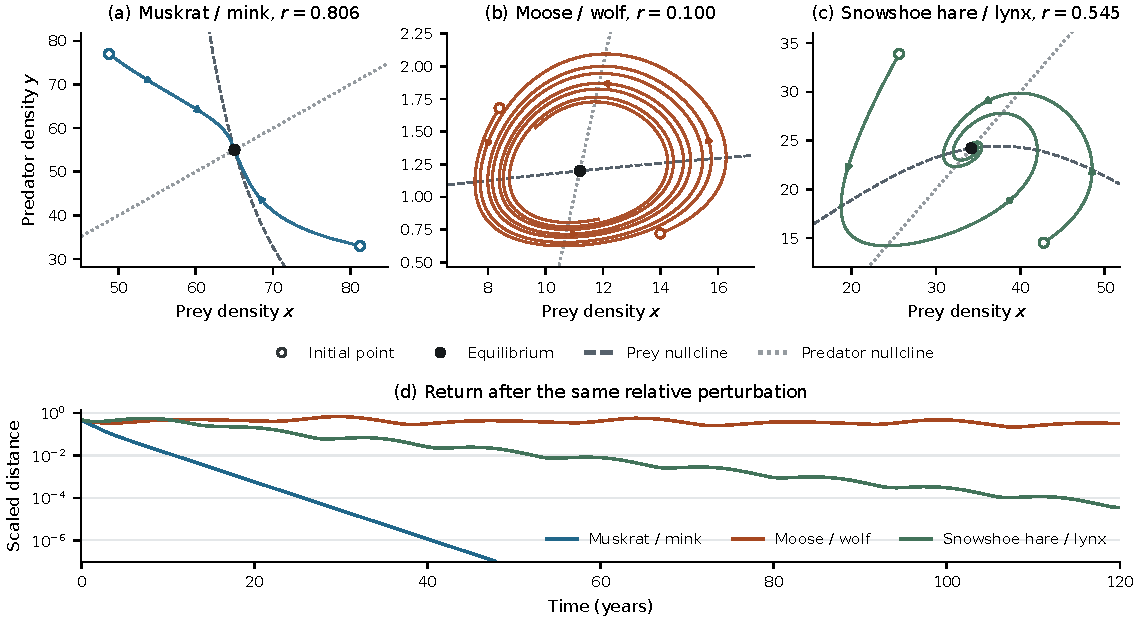
\includegraphics[width=\linewidth]{figures/lit_growth_rates.pdf}
\caption{Growth-rate comparison. Panels (a)--(c) use two initial points,
\((0.75x^*,1.4y^*)\) and \((1.25x^*,0.6y^*)\). Panel (d) shows the Euclidean distance in
\((x/x^*,y/y^*)\) from \((1,1)\) for the first initial point. The time span shown is
120 years. Python source \protect\texttt{code/literature\_cases.py}.}\label{fig:lit-rates}
\end{figure}
